\section{Explaining Type Errors With Traces}
\label{sec:explaining}
%
We have shown how to reliably find witnesses to type errors in \ocaml,
but this not fully address our original goal -- to \emph{explain} the
errors.
%
Having identified an input vector that triggers a bug, a common next
step is to step through the program with a \emph{debugger} to observe
how the program evolves.
%
The existing debuggers and interpreters for \ocaml assume a type-correct
program, so unfortunately we cannot use them off-the-shelf.
%
Instead we return to our semantics for \lang and extend the evaluation
rules to collect a trace that we can present to the user, demonstrating
precisely \emph{how} their program goes wrong.

The trace takes the form of a \emph{reduction graph}, where the nodes
are terms and the edges represent either the single-step
$\hookrightarrow$ or a ``sub-term'' relation. For example, evaluating
the expression @1 + 2 + 3@ would produce the graph in
Figure~\ref{fig:simple-reduction}.
%
\begin{figure}[t]
  \centering
  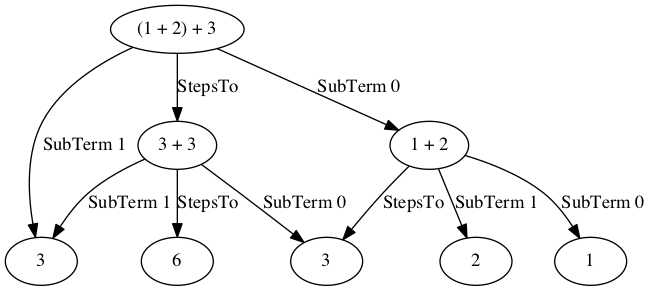
\includegraphics[width=\linewidth]{simple.png}
\caption{The reduction graph for \texttt{1 + 2 + 3}.}
\label{fig:simple-reduction}
\end{figure}

\begin{itemize}
\item extend operational semantics to collect reduction graph
\item nodes are terms, edges indicate ``steps-to'' and ``sub-term'' relations
\item visualize path through reduction graph
\item expand edges to reveal more fine-grained steps (step/jump forward/backward)
\item never lose context (unlike traditional debugger)
\end{itemize}
